\chapter{Website và tùy biến mã nguồn}
\label{ch:web}
\section{Bài toán và tiêu chí nghiệm thu}
Lăng Kính cung cấp không gian trưng bày tác phẩm ảnh/thiết kế, kết hợp xem thư viện công khai với gửi tác phẩm có kiểm duyệt. Khách có thể khám phá theo chủ đề, tác giả hoặc từ khóa; người gửi cần tài khoản phù hợp; Admin/Editor chịu trách nhiệm quyết định xuất bản. Mục tiêu không chỉ là trình bày một lưới ảnh đẹp mà còn duy trì dữ liệu nhất quán từ upload, attachment, tác giả đến trạng thái công khai.

Ranh giới quyền được thiết kế ở phía WordPress. Ẩn nút xuất bản trên giao diện không đủ vì người dùng có thể gọi REST hoặc gửi POST trực tiếp vào wp-admin. Ngược lại, bộ lọc và lightbox là tương tác phía trình duyệt trên danh sách đã được máy chủ giới hạn quyền công khai. Hai nhóm xử lý có vai trò khác nhau: JavaScript hỗ trợ trải nghiệm, còn PHP/capability chịu trách nhiệm cho quy tắc dữ liệu và phân quyền.

\begin{longtable}{P{3.5cm}P{6.1cm}P{4.9cm}}
\caption{Đối chiếu yêu cầu và chức năng hiện có}\label{tab:requirements}\\\toprule Yêu cầu & Hiện thực & Bằng chứng/giới hạn\\\midrule\endfirsthead
\toprule Yêu cầu & Hiện thực & Bằng chứng/giới hạn\\\midrule\endhead
Thư viện số & Trang chủ, 30 ảnh mẫu và tác phẩm thật đã duyệt & Hình \ref{fig:home}; test đếm 30 mẫu khi thêm một bài thật.\\
Album/chủ đề & Taxonomy lk\_topic; album lọc cùng danh sách & Hình \ref{fig:albums}; không tạo bảng DB riêng.\\
Tác giả & post\_author, hiển thị display name và bộ lọc & Bộ lọc ``Bộ sưu tập mẫu'' vẫn trả 30 ảnh.\\
Tìm kiếm & Chuẩn hóa tiếng Việt, tìm trong dữ liệu card & Hình \ref{fig:search}; từ khóa không dấu.\\
Lightbox & Ảnh lớn, trước/sau, Escape, phím mũi tên & Hình \ref{fig:lightbox}; danh sách theo bộ lọc đang dùng.\\
Gửi và duyệt & Shortcode, pending, attachment, featured image & Hai lần gửi tạo hai bài riêng; REST/wp-admin không tự publish.\\
Watermark & Image Watermark; bộ mẫu đã đóng dấu & Hình \ref{fig:watermark}; bản nguồn và backup tách riêng.\\
Tối ưu ảnh & Lazy loading, srcset cho attachment, WebP Nginx & Hình \ref{fig:network}; kiểm tra MIME và fallback.\\
An toàn hệ thống & Module riêng + plugin + template Nginx/PHP & Phần \ref{ch:security}; không coi cài plugin là đủ.\\
Mã nguồn và SQL & Child theme, script bàn giao, SQL clone đã ẩn danh & Có import/restore riêng; không phải backup toàn site.\\\bottomrule
\end{longtable}

\section{Môi trường thực hành và kiến trúc}
Môi trường được đối chiếu trực tiếp gồm Ubuntu 24.04.4, LocalWP 10.2.0, Nginx 1.26.1, PHP 8.2.29, MySQL 8.4.0 và WordPress 7.1.3. Child theme Lăng Kính 2.4.1 có \code{Template: astra}; Astra 4.14.1 là theme cha. Đây là phiên bản đã kiểm chứng của môi trường cụ thể, không phải khuyến nghị đóng băng mọi thành phần ở các phiên bản này khi triển khai lâu dài.

Repo chứa phần tự viết và tài sản đi kèm, không chứa WordPress core, Astra vendor hay toàn bộ plugin. File trong IntelliJ chưa phải file được PHP thực thi. Child theme chạy tại \code{app/public/wp-content/themes/astra-child/}; module bảo mật tại \code{app/public/wp-content/plugins/lang-kinh-security/}. Template Nginx/PHP của LocalWP nằm ngoài document root, sinh thành runtime sau mỗi Stop/Start. Khi thay code phải copy đúng file, so hash và kiểm tra HTTP; khi chỉ thay tài liệu hoặc sanitizer CLI không cần chép các file đó vào website.

\begin{figure}[H]\centering
\begin{tikzpicture}[node distance=9mm,box/.style={draw,rounded corners,align=center,text width=4.2cm,minimum height=12mm,font=\small},>=Stealth]
\node[box] (client) {Trình duyệt\\Khách / Author / Editor / Admin};
\node[box,below=of client] (nginx) {Nginx LocalWP\\static, WebP, chặn endpoint};
\node[box,below=of nginx] (wp) {PHP-FPM + WordPress\\Child theme + plugin/module};
\node[box,below left=10mm and 3mm of wp] (db) {MySQL\\post, meta, taxonomy, user};
\node[box,below right=10mm and 3mm of wp] (disk) {Filesystem\\uploads, ảnh mẫu, WebP};
\draw[->] (client)--(nginx);\draw[->] (nginx)--(wp);\draw[<->] (wp)--(db);\draw[<->] (wp)--(disk);
\end{tikzpicture}
\caption[Sơ đồ thiết kế kiến trúc]{Sơ đồ thiết kế kiến trúc do nhóm biên soạn; không phải ảnh chụp hoạt động hay sơ đồ mạng production.}\label{fig:architecture}
\end{figure}

\section{Trang chủ, banner và responsive}
Trang chủ dùng \code{front-page.php}; CSS của child theme định nghĩa vùng hero, card, album, bộ lọc và các breakpoint. Thiết kế hiện tại được giữ nguyên, không thay Astra hay chuyển sang page builder. Banner cố định lấy từ cấu hình Customizer trong \code{inc/hero.php}; khi chưa cấu hình có fallback đến ảnh mẫu đã watermark. Việc thêm bài mới chỉ bổ sung card đầu danh sách, không thay ảnh đại diện nhận diện website.

Người dùng vào trang chủ có thể xem banner, chọn ``Khám phá tác phẩm'' hoặc chuyển tới album. Mobile thay số cột và kích thước phần tử để tránh cuộn ngang. Kiểm thử tại 390 px và 1440 px kiểm tra chiều rộng document, khả năng decode ảnh và mở lightbox. Kiểm tra bằng ảnh chụp không thay cho việc đo overflow bằng JavaScript, nên cả hai loại bằng chứng được dùng cùng nhau.
\shot{home-desktop.png}{Trang chủ LocalWP thật, chụp ngày 27/10/2026. Quan sát bố cục hero, banner cố định và liên kết gửi tác phẩm; nguồn: trình duyệt Edge.}{fig:home}


\section{Album, chủ đề và tác giả}
\noindent\begin{minipage}[t]{0.32\linewidth}\vspace{0pt}\centering
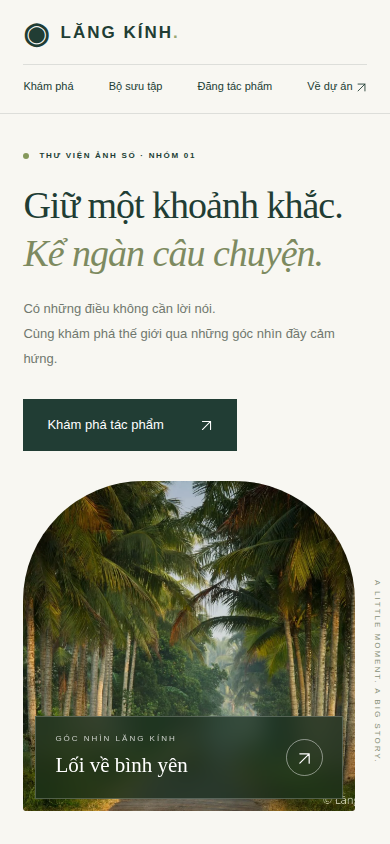
\includegraphics[width=0.9\linewidth,height=0.40\textheight,keepaspectratio]{figures/home-mobile.png}
\captionof{figure}[Trang chủ mobile]{Trang chủ ở viewport 390 px trên LocalWP thật. Nguồn: Edge headless; ảnh minh họa kiểm tra responsive, không thay thế kiểm thử trên mọi thiết bị vật lý.}\label{fig:mobile}
\end{minipage}\hfill
\begin{minipage}[t]{0.64\linewidth}\vspace{0pt}
Mỗi tác phẩm là một bài \code{lk_photo}; chủ đề là taxonomy phân cấp \code{lk_topic}. Những album trên trang chủ sử dụng cùng các slug chủ đề, nhờ vậy chọn album và chọn chip chủ đề có thể tác động lên cùng tập card. Các chủ đề của ảnh mẫu được khai báo trong catalog và seed có phiên bản, không nhập lại 30 bài mẫu vào DB trên mỗi lượt xem.

Form tải danh sách chủ đề hiện có từ taxonomy. Nếu không chọn, hệ thống dùng ``Tự do''. Chọn ``Khác'' yêu cầu tên mới tối đa 80 ký tự; server tìm lại term đã tồn tại trước khi tạo. Term mới chỉ được tạo sau khi ảnh/bài đã lưu hợp lệ, giúp tránh tích lũy term từ request thất bại. Quy tắc này không có nghĩa Author được quản trị tùy ý mọi taxonomy trong wp-admin; đây là hành vi giới hạn trong luồng gửi tác phẩm.

Tác giả của bài thật lấy từ WordPress, không tin tên tác giả tự gửi trong POST. Ảnh mẫu có nhãn riêng ``Bộ sưu tập mẫu''. Sau khi lọc tác giả mẫu, số card phải luôn là 30 ngay cả khi có bài thật. Với tài khoản bị xóa hoặc đổi tên, quản trị viên cần xử lý quyền sở hữu bằng chức năng WordPress; code không tự thay danh tính tài khoản thật.
\end{minipage}

\shot{albums.png}{Khu vực album trên trang chủ LocalWP. Nguồn: ảnh chụp thật; chọn album dùng cùng cơ chế lọc chủ đề của lưới.}{fig:albums}

\section{Tìm kiếm và lightbox}
JavaScript trong \code{js/custom.js} chuẩn hóa chuỗi về chữ thường, loại dấu tổ hợp và xử lý chữ đ/Đ để hỗ trợ từ khóa không dấu. Danh sách card hiện có được lọc theo điều kiện chủ đề, tác giả và từ khóa. Không có request SQL tìm kiếm riêng cho mỗi lần gõ; cách này phù hợp dữ liệu demo nhỏ, nhưng với số lượng lớn cần phân trang/query phía máy chủ thay vì tải toàn bộ bài một lần.

Sau khi lọc, số lượng, trạng thái ``không tìm thấy'' và các lớp chiều cao card được cập nhật theo những phần tử đang hiển thị. Điều chỉnh CSS focus cho ô tìm kiếm giúp khung không bị lệch khi nhập. Các trạng thái focus bàn phím vẫn được giữ để người dùng nhận biết điều khiển hiện tại. Không dùng việc bỏ toàn bộ outline như giải pháp sửa hình thức.
\shot{search.png}{Tìm ``huong mua ha'' không dấu trên LocalWP trả đúng ảnh ``Hương mùa hạ''. Nguồn: trình duyệt thật; ảnh quan sát ô nhập, kết quả và bộ lọc.}{fig:search}

Lightbox hiển thị ảnh đầy đủ từ thuộc tính dữ liệu của card. Danh sách trước/sau được lấy từ kết quả đang thấy, tránh chuyển sang ảnh đã bị bộ lọc ẩn. Người dùng có thể dùng nút điều hướng, phím mũi tên, Escape hoặc nút đóng; focus được quản lý khi mở/đóng. CSS đã sửa khung vuông trắng ở nút đóng và điều hướng, không thay ảnh gốc để che lỗi giao diện. Kiểm thử còn kiểm tra ảnh trong hộp xem đã decode và không gây overflow mobile.
\shot{lightbox.png}{Lightbox LocalWP ở kết quả tìm kiếm. Nguồn: Edge; quan sát nền tối, ảnh lớn và điều khiển đóng/chuyển.}{fig:lightbox}

\section{Gửi tác phẩm và vòng đời dữ liệu}
\subsection{Shortcode và xử lý trước HTML}
Trang \code{/dang-tac-pham/} chứa shortcode \code{[lk_upload_form]}. Shortcode chỉ dựng giao diện; hook \code{template_redirect} xử lý request trước khi template xuất HTML. Khách nhận liên kết đăng nhập do \code{wp_login_url} tạo, có đích quay lại form và tự tương thích WPS Hide Login. Người đã đăng nhập nhưng thiếu \code{upload_files} hoặc \code{edit_lk_photos} vẫn bị từ chối.

Sau kiểm tra quyền, server xác minh nonce, tiêu đề, chủ đề và file. MIME phải khớp loại ảnh thực từ file tạm, không chỉ dựa vào phần mở rộng hoặc Content-Type do trình duyệt khai. Phần upload dùng API media WordPress, tạo attachment và các kích thước ảnh, sau đó tạo \code{lk_photo} với status pending và author là tài khoản hiện tại. Thumbnail phải gắn thành công mới được coi là tác phẩm hoàn chỉnh.

Nếu tạo bài, thumbnail hoặc gán chủ đề thất bại, code dọn bài/attachment vừa tạo trong request đó; không xóa ảnh đại diện người dùng đã chọn trước đây. Khi hoàn tất, response 303 chuyển về GET có receipt gắn bài/tài khoản. Thông báo thành công được kiểm tra bằng nonce receipt, owner, status và thumbnail, không chỉ nhìn chuỗi \code{lk_upload=pending}.
\shot{upload-form.png}{Form của tài khoản thử dùng một lần trên LocalWP; các mục chủ đề lấy từ taxonomy. Nguồn: ảnh chụp thật, không phải wireframe.}{fig:uploadform}
\shot{upload-pending.png}{Thông báo sau khi request thực sự lưu thành công bài/ảnh chờ duyệt. Nguồn: LocalWP; dữ liệu thử đã được dọn sau kiểm thử.}{fig:pending}

\subsection{Sửa lỗi gửi lần hai và giới hạn PHP}
Lỗi cũ xuất hiện khi code ưu tiên tham số GET thông báo trước POST: lần hai gửi từ URL có pending chỉ hiện thành công nhưng không lưu dữ liệu. Bản hiện tại ưu tiên xử lý POST, form action là permalink sạch và sử dụng Post/Redirect/Get. Test gửi hai lần liên tiếp yêu cầu hai ID khác nhau, cùng pending và đều có featured media; chỉ thấy hai thông báo xanh không đủ chứng minh yêu cầu này.

Một lỗi khác xuất hiện trước khi WordPress chạy: PHP có thể làm rỗng cả POST và FILES khi body vượt \code{post_max_size}. Do đó handler so Content-Length với giới hạn tổng POST trước điều kiện kiểm tra nút submit. K/M/G dùng hệ số nhị phân; 0 hoặc giá trị âm được xử lý là không giới hạn tổng trong helper. Request quá lớn nhận 413 và hướng dẫn nhập lại/chọn ảnh nhỏ hơn, không chuyển thành công. Giới hạn 12 MB của form khác giới hạn tệp PHP và khác giới hạn tổng request.\cite{phpLimits}

Trên LocalWP thật đã tạm đặt post limit 16 MB, gửi request 17 MB và nhận 413; sau đó khôi phục đúng template PHP 1000 MB ban đầu và Stop/Start. Tệp 13 MB bị chặn bởi giới hạn form ngay cả khi server cho phép lớn hơn. PHP ghi một cảnh báo do phép thử cố tình vượt giới hạn; đây không phải lỗi fatal trong code. Kết quả được tách khỏi tuyên bố ``không có lỗi ngoài dự kiến''.

\subsection{Phân quyền và duyệt}
CPT dùng bộ capability \code{lk_photo/lk_photos} và \code{map_meta_cap=true}. Author có quyền tạo/sửa tác phẩm phù hợp nhưng không có publish capability của CPT; Admin/Editor có quyền xem và duyệt pending. Không xóa \code{publish_posts} trên toàn WordPress vì việc đó làm thay đổi quyền bài viết thông thường ngoài phạm vi thư viện.\cite{wordpressCpt}

Test Author cố tạo publish/future/private qua REST nhận 403, sửa pending thành publish cũng bị chặn; POST vào wp-admin không tự xuất bản được. Editor đọc được bài pending có thumbnail và chuyển publish thành công. Khi đó trang chủ thêm một bài thật trước 30 ảnh mẫu. Một bài draft/pending/trash hoặc không có thumbnail hợp lệ không được đưa vào danh sách công khai.
\shot{moderation.png}{Danh sách tác phẩm trong wp-admin của tài khoản kiểm duyệt thử. Nguồn: LocalWP thật; các bài thử minh họa pending và published, không phải nội dung của tài khoản thật.}{fig:moderation}

\section{Watermark và tối ưu ảnh}
\subsection{Watermark, bản gốc và backup}
Image Watermark 2.0.16 được cấu hình tự áp dụng cho ảnh upload, ở frontend và admin theo kích thước được chọn. Nội dung dấu ``© Lăng Kính · Nhóm 1'' dùng font hỗ trợ tiếng Việt. Plugin có cơ chế backup ảnh trước xử lý; dữ liệu backup nằm ngoài repo và không được nhầm với ảnh đang phục vụ công khai. Khi thay cấu hình watermark phải kiểm tra ảnh đầu ra, tránh chồng nhiều dấu hoặc tạo WebP từ file chưa đóng dấu.

Bộ 30 ảnh mẫu dùng các file đã watermark trong \code{assets/demo-watermarked/}; bản nguồn giữ riêng và manifest có checksum. Ảnh mẫu không tự trở thành attachment trong DB. Việc đóng watermark không chuyển quyền tác giả của ảnh gốc sang nhóm; hồ sơ nguồn ảnh vẫn là yêu cầu pháp lý/tài liệu còn thiếu. Không dùng dấu của nhóm để khẳng định sở hữu ảnh chưa có chứng cứ.
\shot[0.75]{watermark-new.png}{Vùng watermark trên WebP của ảnh mới upload trong kiểm thử LocalWP. Nguồn: crop từ file derivative thật; crop chỉ để đọc dấu, không thêm chữ vào ảnh.}{fig:watermark}

Lazy loading trì hoãn tải những card ngoài vùng xem; banner được ưu tiên tải. Bài thật có srcset/sizes do WordPress sinh từ attachment metadata, giúp trình duyệt chọn kích thước phù hợp viewport. Ảnh mẫu hiện dùng file cố định nên không tuyên bố chúng có đầy đủ srcset như attachment. WebP giảm định dạng truyền tải theo khả năng client; không thay thế việc giới hạn kích thước pixel, nén hợp lý hoặc kiểm tra chất lượng.

\subsection{Chẩn đoán và sửa WebP trên Nginx}
Converter for Media 6.7.0 trước đây bật Pass Thru với cả uploads và themes. Chẩn đoán thực tế xác nhận URL loader cho ảnh theme trả HTTP 200, Content-Type HTML và body rỗng, trong khi JPG trực tiếp vẫn mở được. Đọc mã plugin cho thấy bộ đổi URL áp dụng cho thư mục themes nhưng allowlist của Pass Thru chỉ map uploads. Vì vậy nguyên nhân được kết luận từ cả HTTP lẫn source; không đoán rằng mọi file JPG đã mất hoặc tự thay phần mở rộng hàng loạt.

Giải pháp hiện tại giữ Converter bật và dùng chế độ rewrite. Tên tùy chọn loader là \code{htaccess}, nhưng Nginx không đọc file .htaccess; quy tắc tương đương được đặt trong template LocalWP. Snippet nằm trước các regex ảnh/include khác, tìm derivative trong uploads-webpc khi Accept có WebP và fallback về URI gốc nếu không có file. Response có Vary: Accept để cache không nhầm bản JPG và WebP. Cấu hình tham khảo hướng dẫn chính thức của plugin, giới hạn thư mục uploads/themes và không bật AVIF trong đợt này.\cite{converterNginx}
\shot{network-webp.png}{DevTools Network thật của Edge gắn với LocalWP: cùng URL JPG, response image/webp khi gửi Accept WebP. Nguồn: DevTools trực tiếp, không dựng lại bảng Network.}{fig:network}
\shot{network-fallback.png}{DevTools Network thật khi gửi Accept image/jpeg: URL giữ nguyên, response image/jpeg và Vary: Accept. Nguồn: cùng phiên kiểm chứng LocalWP.}{fig:fallback}

Các trường quan trọng được chép ra bảng để đọc khi in A4; ảnh Network độ phân giải đầy đủ được giữ trong thư mục figures. Đây là số liệu HTTP thực, không phải bảng giả làm screenshot.
\begin{table}[H]\centering\small
\caption{Đối chiếu negotiation cho cùng URL ảnh banner}
\begin{tabularx}{\linewidth}{YYY}\toprule Trường & Client WebP & Client JPEG\\\midrule
Accept & image/webp & image/jpeg\\
HTTP / Content-Type & 200 / image/webp & 200 / image/jpeg\\
Vary & Accept & Accept\\
Body & Khớp derivative WebP trên đĩa & Khớp JPG nguồn trên đĩa\\\bottomrule
\end{tabularx}\end{table}

Đã kiểm tra 30 ảnh mẫu và 14 biến thể của hai ảnh mới, mỗi file theo hai Accept, tổng 88 request: status, MIME, Vary và body khớp file tương ứng trên đĩa. Khi thiếu derivative, client hỗ trợ WebP vẫn nhận JPG hợp lệ. Ảnh mới có cờ watermark, đầy đủ derivative và dấu còn nhìn thấy trên WebP. Kiểm tra trang sau Stop/Start xác nhận template sinh lại và trình duyệt decode ảnh/banner/lightbox ở desktop/mobile. Không gọi việc chỉ tắt plugin là hoàn tất WebP.

\section{Tổ chức code tự viết}
\subsection{Nạp tài nguyên và khai báo mô hình}
\code{functions.php} đăng ký theme support, kích thước lk-gallery, enqueue CSS/JS, CPT và taxonomy; phần upload và banner tách sang inc để dễ đọc và kiểm thử. Version tài nguyên dùng mtime của file tự viết; version Astra giữ theo theme cha để cache busting. Không xóa bừa mọi query ver nhằm che dấu phiên bản.

Trích đoạn đang dùng để nạp tài nguyên:
\sourcefile{astra-child/functions.php}{11}{15}
Trích đoạn cấu hình riêng quyền và liên kết taxonomy:
\sourcefile{astra-child/functions.php}{21}{27}

Lớp giao diện không cấp quyền dựa trên role name nhận từ client. Phân quyền thực tế dùng capability của WordPress; migration chạy tại init với marker phiên bản, bổ sung quyền và tạo trang còn thiếu ngay cả khi theme đã active từ trước. Nếu trang do người dùng tạo đã tồn tại, code không ghi đè nội dung. Migration chỉ ghi marker hoàn tất khi seed/chức năng tạo trang trả thành công.

\subsection{Danh sách kết hợp và xử lý lỗi}
\code{lk_gallery_items()} query riêng publish, bỏ qua bài thiếu thumbnail/src, dựng trường tác giả/chủ đề/srcset rồi nối catalog mẫu. Cách này giữ thứ tự bài thật trước và làm số lượng/bộ lọc/lightbox làm việc trên một tập thống nhất. Query không phân trang phù hợp demo; mở rộng production cần xem xét số lượng bài, bộ nhớ và phương pháp tìm kiếm.

Handler upload có đường thoát rõ khi gặp sai nonce, chủ đề, MIME, kích thước hoặc lỗi lưu. Server là lớp bắt buộc, bởi JavaScript có thể bị tắt/bỏ qua. Receipt thành công không cho người dùng đọc tùy ý pending của người khác. Cơ chế dọn chỉ nhắm ID vừa tạo trong cùng luồng, tránh xóa attachment hiện hữu vì một request giả mạo.

Back-to-top và các thao tác menu/scroll được xử lý trong JavaScript của child theme; chúng không thay đổi trạng thái server. Khi người dùng yêu cầu giảm chuyển động, CSS tôn trọng prefers-reduced-motion. Phạm vi kiểm thử giao diện gồm viewport desktop/mobile, trạng thái tìm rỗng, lọc tác giả, album, mở/đóng lightbox và không có lỗi JavaScript ngoài dự kiến.

\section{Git, thành phần bên thứ ba và license}
Nhóm phát triển trên nhánh huyyhoangg, kiểm tra HEAD và working tree trước sửa; không reset toàn repo hoặc sửa lịch sử để gán đóng góp. Repo nộp cuối cần được điền sau khi nhóm tự review. Lượt chuẩn hóa này không tự commit/push/merge; người phụ trách xem diff, chạy test và quyết định commit theo phần việc thực tế. Không tạo commit giả chỉ để đủ năm tên trong danh sách.

\begingroup\small\setlength{\tabcolsep}{3pt}
\begin{longtable}{P{3.4cm}P{1.2cm}P{2.4cm}P{2.7cm}P{4.1cm}}
\caption{Kiểm kê đầy đủ core, theme và plugin cài trên LocalWP}\label{tab:plugins}\\\toprule Tên & Phiên bản & Trạng thái & License & Mục đích\\\midrule\endfirsthead
\toprule Tên & Phiên bản & Trạng thái & License & Mục đích\\\midrule\endhead
WordPress & 7.1.3 & Core & GPL-2.0-or-later & Nền tảng nội dung\\
Astra & 4.14.1 & Theme cha & GPL-2.0-or-later & Theme nền\\
Lăng Kính Child & 2.4.1 & Đang dùng & GPL-2.0-or-later & Giao diện/CPT/shortcode\\
Twenty Twenty-Five & 1.5 & Không active & GPL-2.0-or-later & Theme mặc định\\
Twenty Twenty-Four & 1.6 & Không active & GPL-2.0-or-later & Theme mặc định\\
Twenty Twenty-Three & 1.7 & Không active & GPL-2.0-or-later & Theme mặc định\\
Image Watermark & 2.0.16 & Active & MIT & Watermark/backup ảnh\\
Converter for Media & 6.7.0 & Active, rewrite & GPL-2.0-or-later & WebP Nginx/fallback\\
Wordfence Security & 9.0.2 & Active, Basic & GPL-3.0-or-later & WAF; không xác nhận Premium\\
LLAR & 3.3.10 & Active, free/local & GPL-2.0-or-later & Giới hạn đăng nhập\\
WPS Hide Login & 1.9.19 & Active & GPL-2.0-or-later & URL đăng nhập riêng\\
Lăng Kính Security & 1.0.0 & Active & GPL-2.0-or-later & Module nhóm tự viết\\
\bottomrule\end{longtable}\endgroup
Nguồn kiểm chứng: header style.css của từng theme; header/readme của plugin đã cài; directory chính thức WordPress.org. Bảng không có key/license token. Bản miễn phí và trạng thái active không đồng nghĩa có quyền Premium. Xem PLUGIN-LICENSES.md để tra URL nguồn từng gói.\cite{plugins}


WordPress/Astra/plugin chính thức được cài ngoài repo từ nguồn tương ứng. Module \code{security/lang-kinh-security/} và child theme là phần nhóm quản lý, không phải phiên bản sửa của vendor. LICENSE MIT gốc vẫn giữ nguyên thông báo hiện hữu; phạm vi GPL được ghi ở header các thành phần riêng. Hồ sơ license phải được rà lại khi cập nhật gói, vì inventory ghi nhận thời điểm khảo sát, không phải chứng nhận vĩnh viễn.
